\chapter{FIREBALL}
\section{Introducción al código FIREBALL}
Consiste en un procedimiento basado en el formalismo de electrones fuertemente ligados (\emph{tight-binding}) y de dinámica molecular, parametrizada con datos \emph{ab-initio}. Se procede a realizar un cálculo de DFT usando orbitales atómicos (LCAO) modificados para cortarlos a un determinado valor de la distancia al núcleo, a partir del cual la f.d.o se hace nula. \\

% \coffeestainD{0.5}{0.85}{-25}{5cm}{1.3cm} 

Por otro lado, se usa la aproximación de McWeeda para modelizar la energía de correlación y canje.
\section{Cálculos con FIREBALL: resultados}
\subsection{Grafeno 1x1: energías frente parámetro de red}
\begin{figure}[!h]
    \centering
    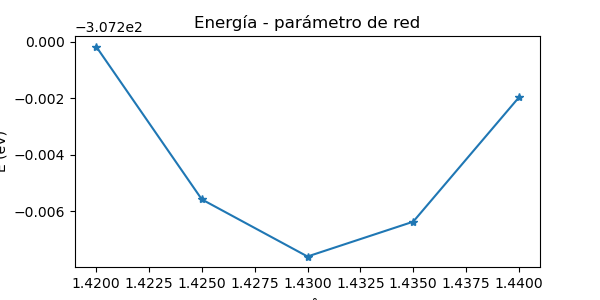
\includegraphics[scale=.8]{FIGURAS/En_param_graf1x1.png}
    \caption{$E$ (eV) frente a $a$ (\AA)}
    \label{fig:enter-label}
\end{figure}



El parámetro de red $a$ que tiene asociada la energía más pequeña es $a = 1.43 $ \AA, con $E_{TOT} = -307.207591$ eV.
\subsection{Densidad de estados frente a energía}
\begin{figure}[!h]
    \centering
    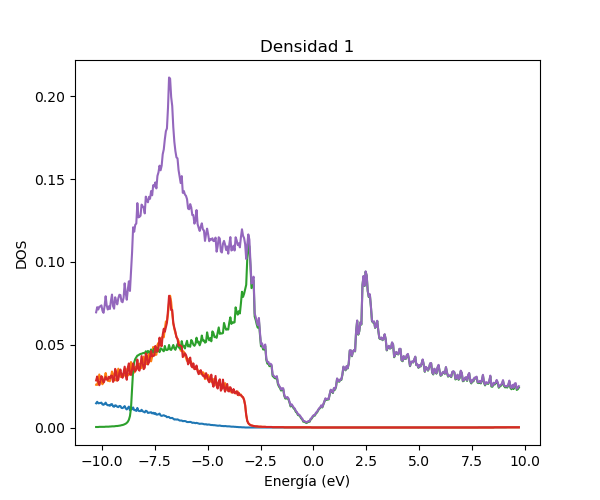
\includegraphics[scale=.6]{FIGURAS/Densidad_1.png}
    \caption{DOS frente a $E$ (eV)}
    \label{fig:enter-label}
\end{figure}
\begin{figure}[!h]
    \centering
    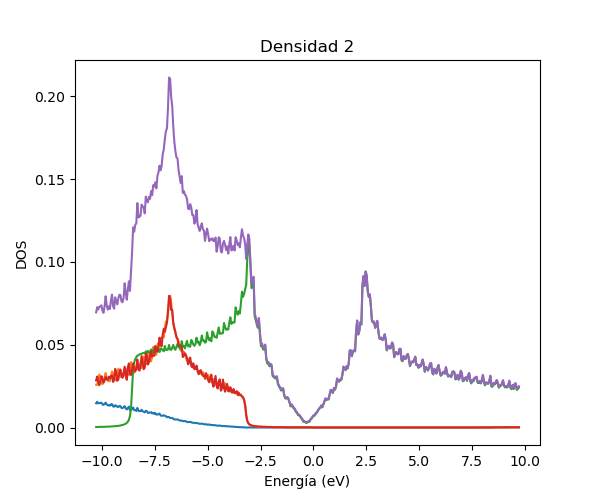
\includegraphics[scale=.6]{FIGURAS/Densidad_2.png}
    \caption{DOS frente a $E$ (eV)}
    \label{fig:enter-label2}
\end{figure}
\begin{figure}[!t]
    \centering
    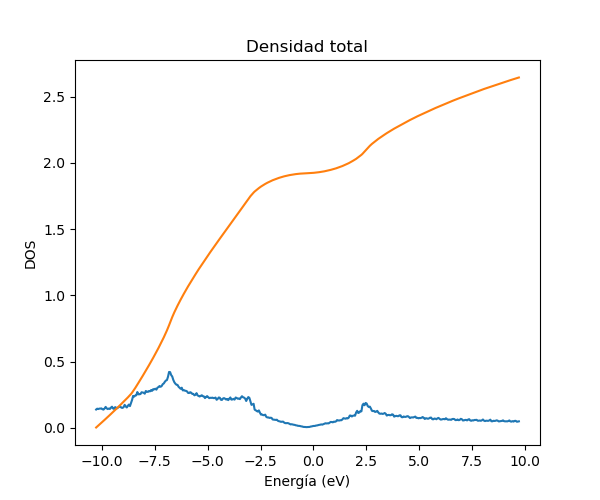
\includegraphics[scale=.6]{FIGURAS/Densidad_total.png}
    \caption{DOS frente a $E$ (eV)}
    \label{fig:enter-label3}
\end{figure}
\clearpage 
\section{Grafeno 18x8. Estiramiento, energía y fuerzas}

% \begin{figure}[!h]
%     \centering
%     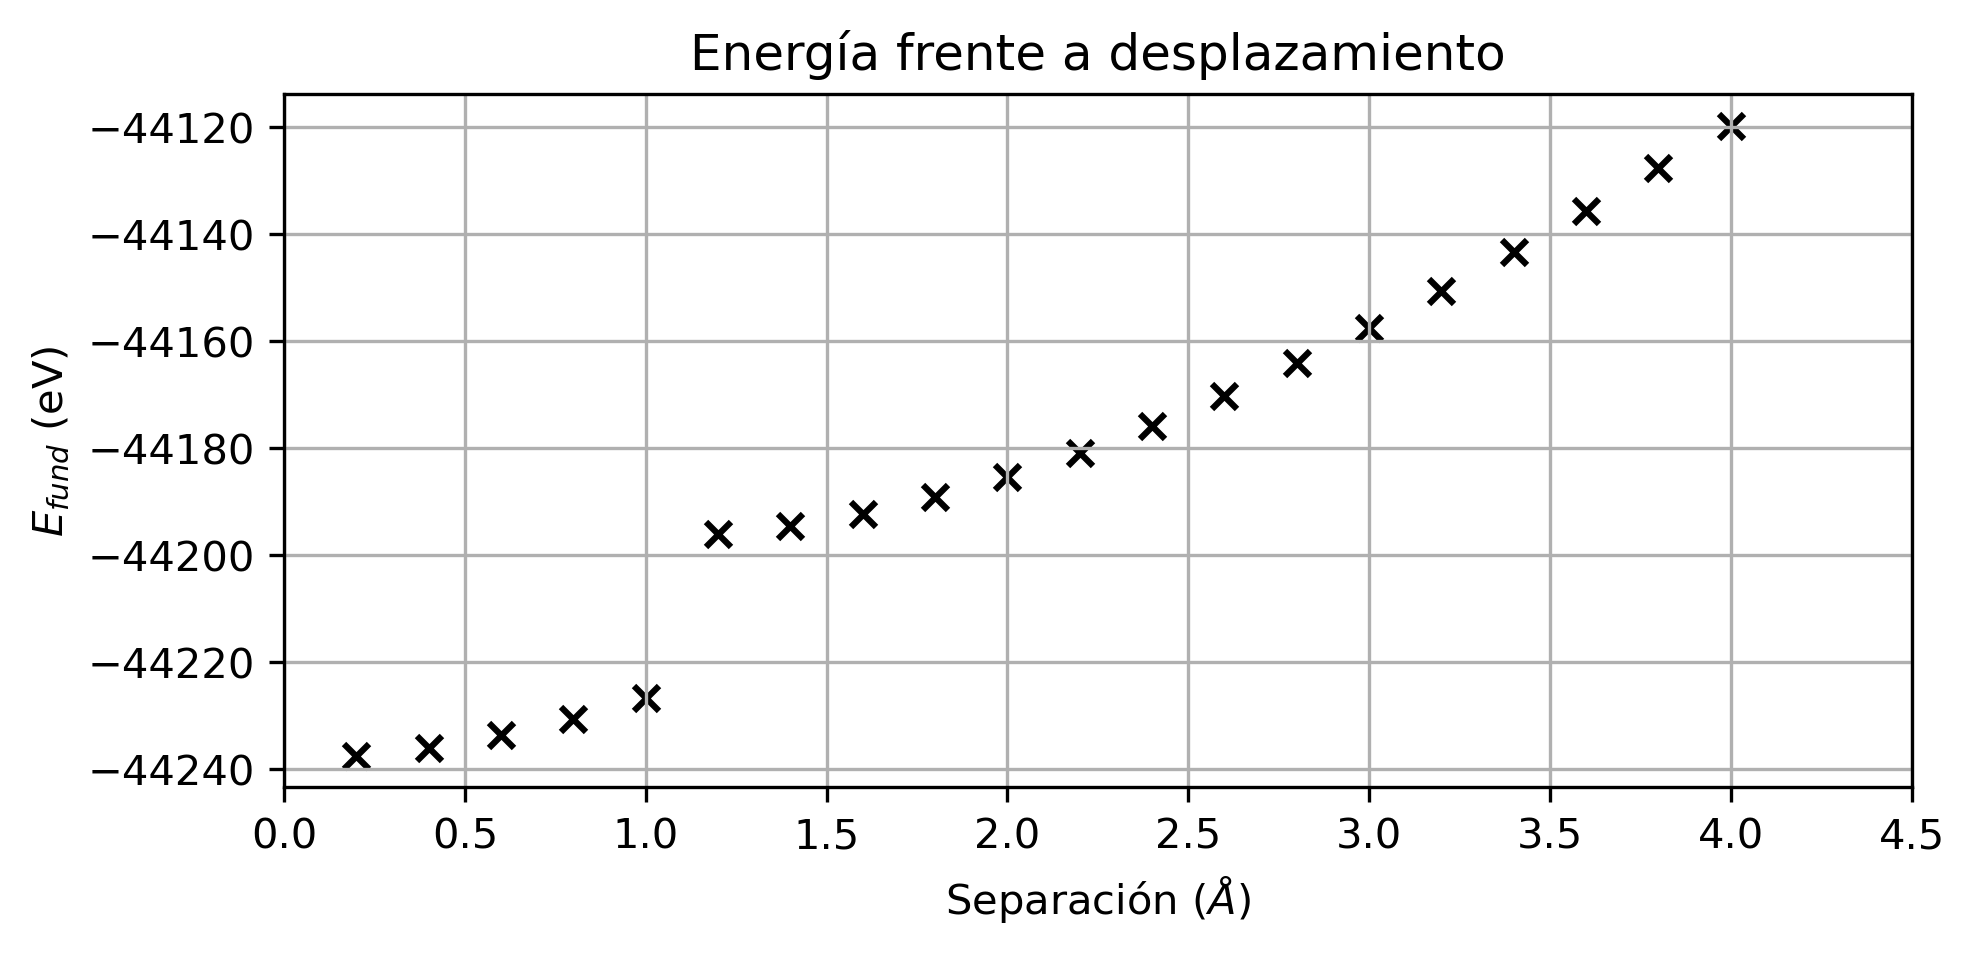
\includegraphics[scale = .9]{FIGURAS/E_desp_graf_18x8.png}
%     \label{fig:graf_18x8}
% \end{figure}

\begin{figure}[!h]
    \centering
    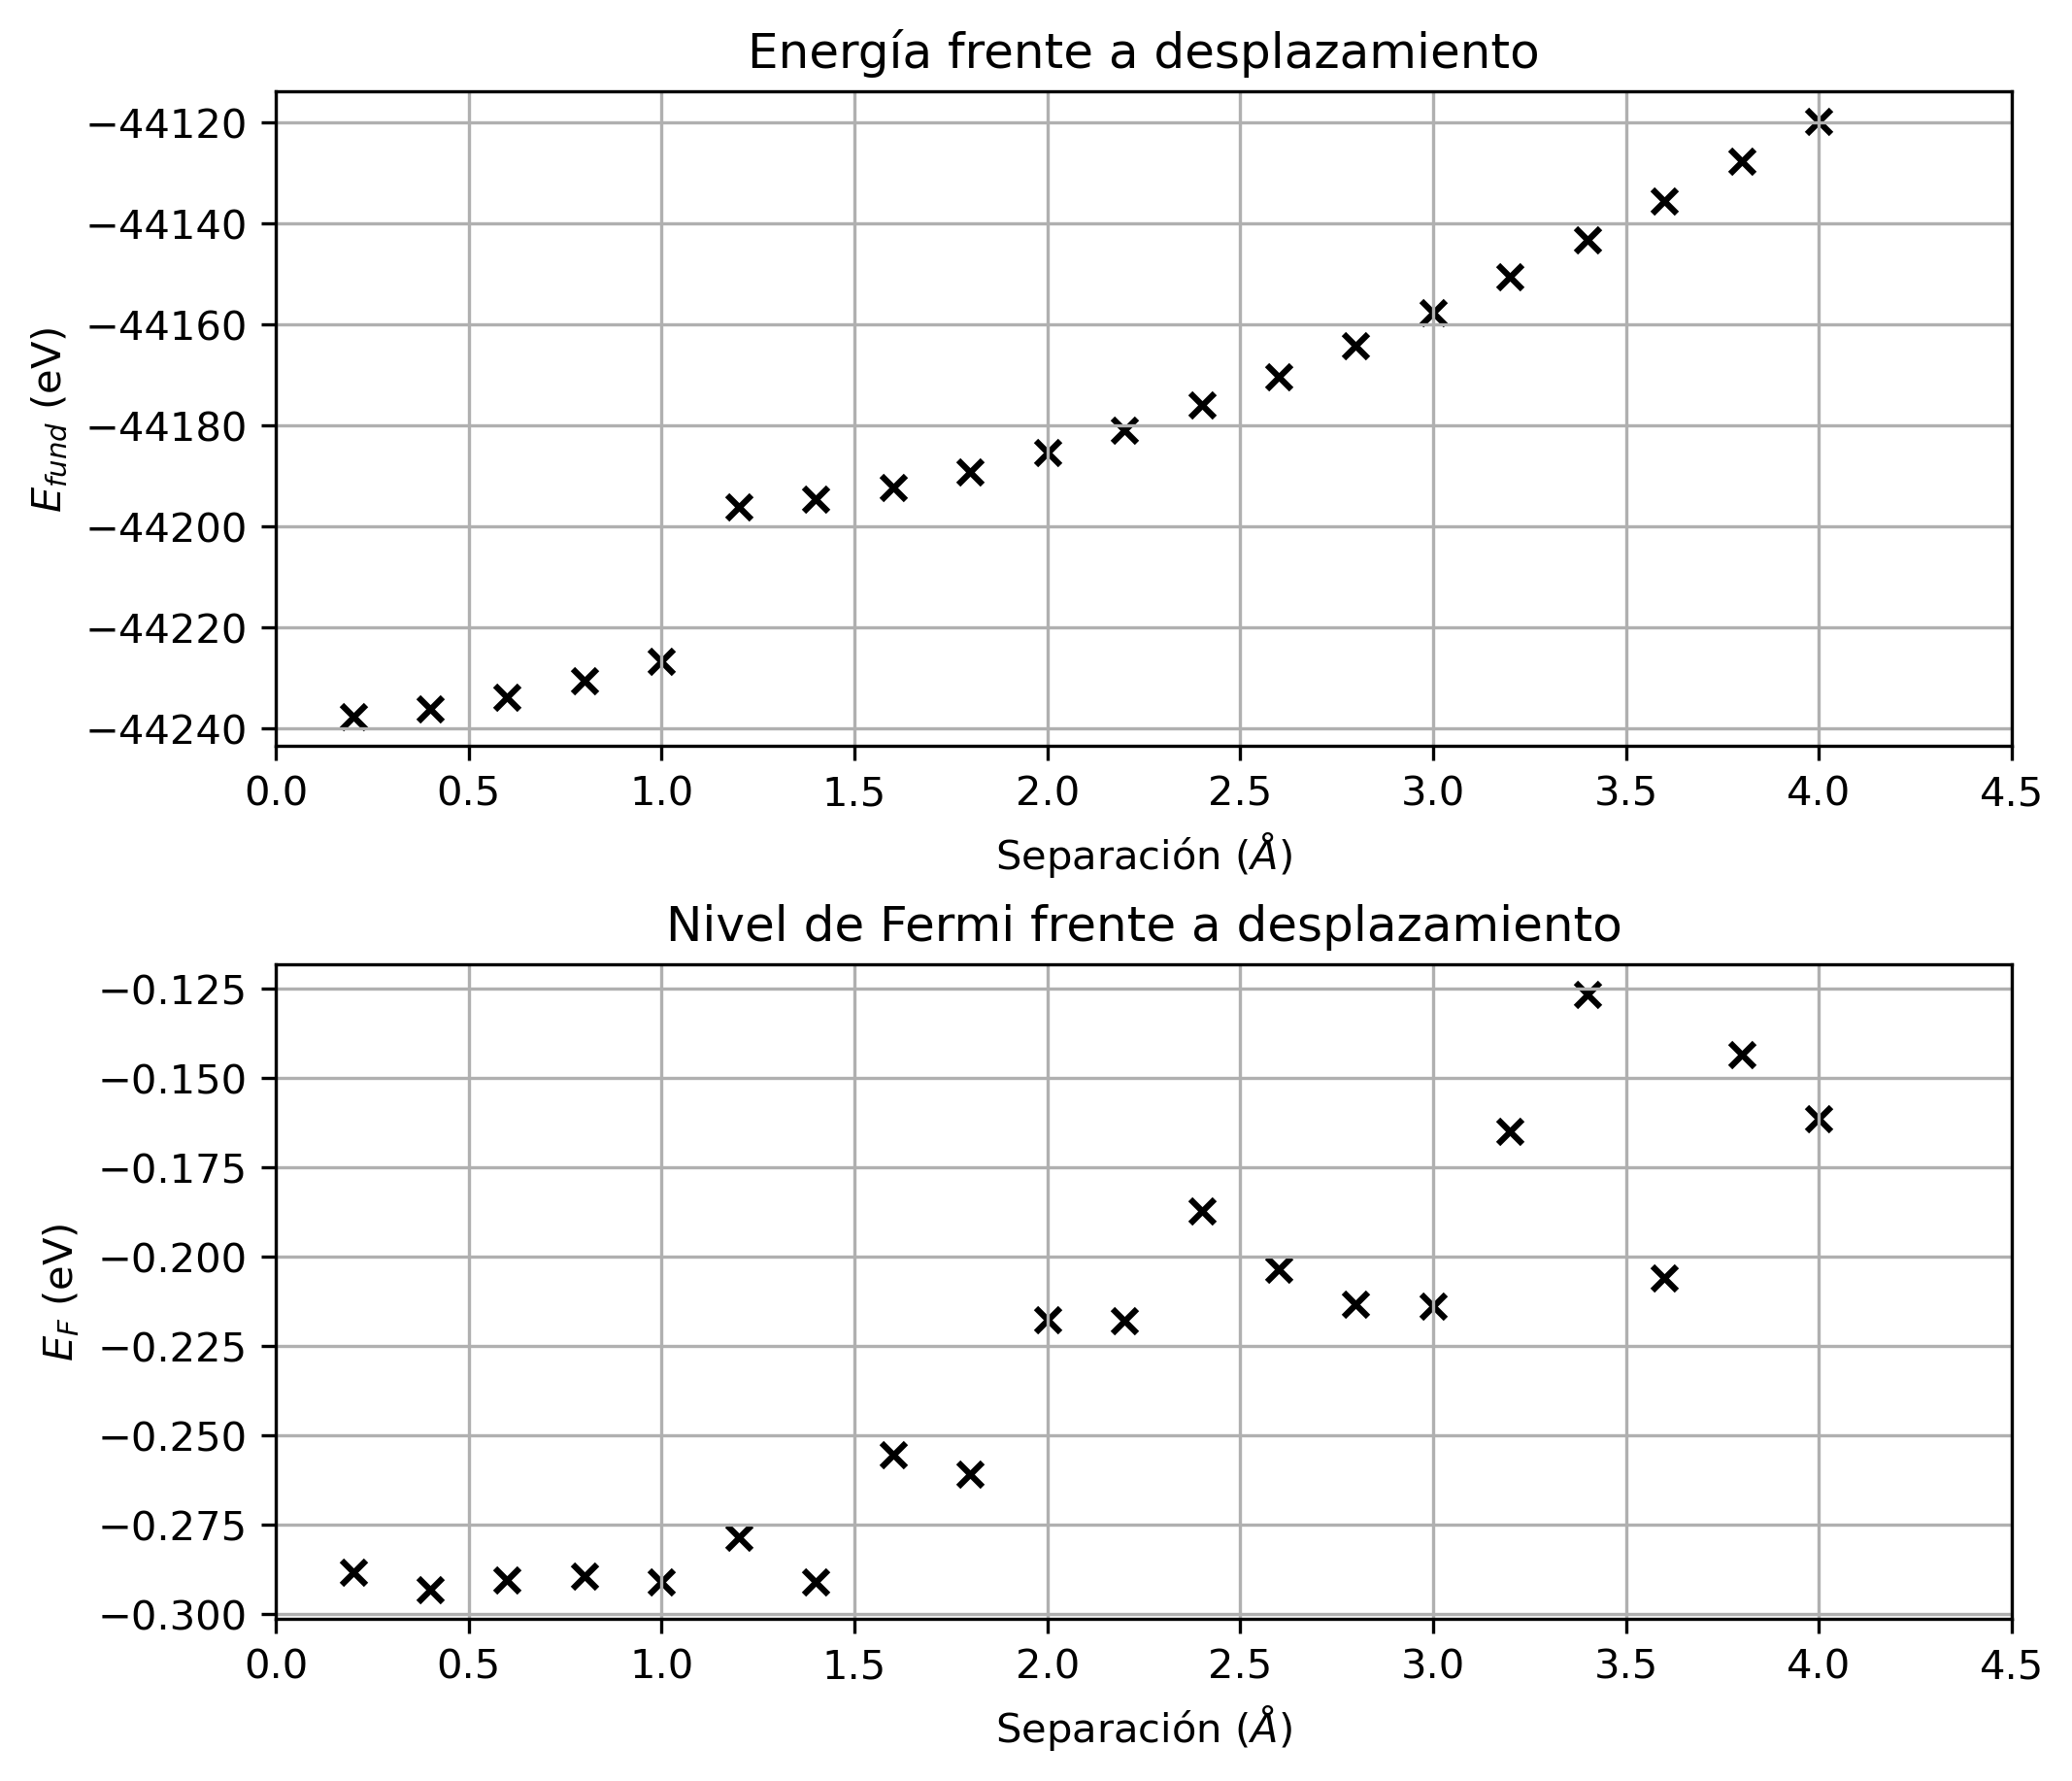
\includegraphics[scale = .9]{FIGURAS/E_F_desp_graf_18x8.png}
    \label{fig:18x8_e_ef}
\end{figure}

Rehacer las figuras

\begin{itemize}
    \item El grafeno se rompe por uno de los extremos. Es más estable romper por los extremos.
    \item Al realizar un estiramiento progresivo de la red, observamos que la configuración de mínima energía es muy distinta a la obtenida al estirar rígidamente por los extremos. 
\end{itemize}

\section{Grafeno 18x8 vacante y divacante}

\begin{itemize}
    \item Al haber una vacante, es más estable que el grafeno se rompa por el defecto antes que por la región en la que estiramos. 
    \item Ocurre lo mismo con la divacante. 
    \item En ambos casos, la configuración de mínima energía hace que los átomos de la región de ruptura salgan del plano del grafeno. 
\end{itemize}


\section{Conlusiones}

\begin{itemize}
    \item Importa el tipo de defecto que introducimos.
    \item Importa la manera en la que estiramos. 
\end{itemize}

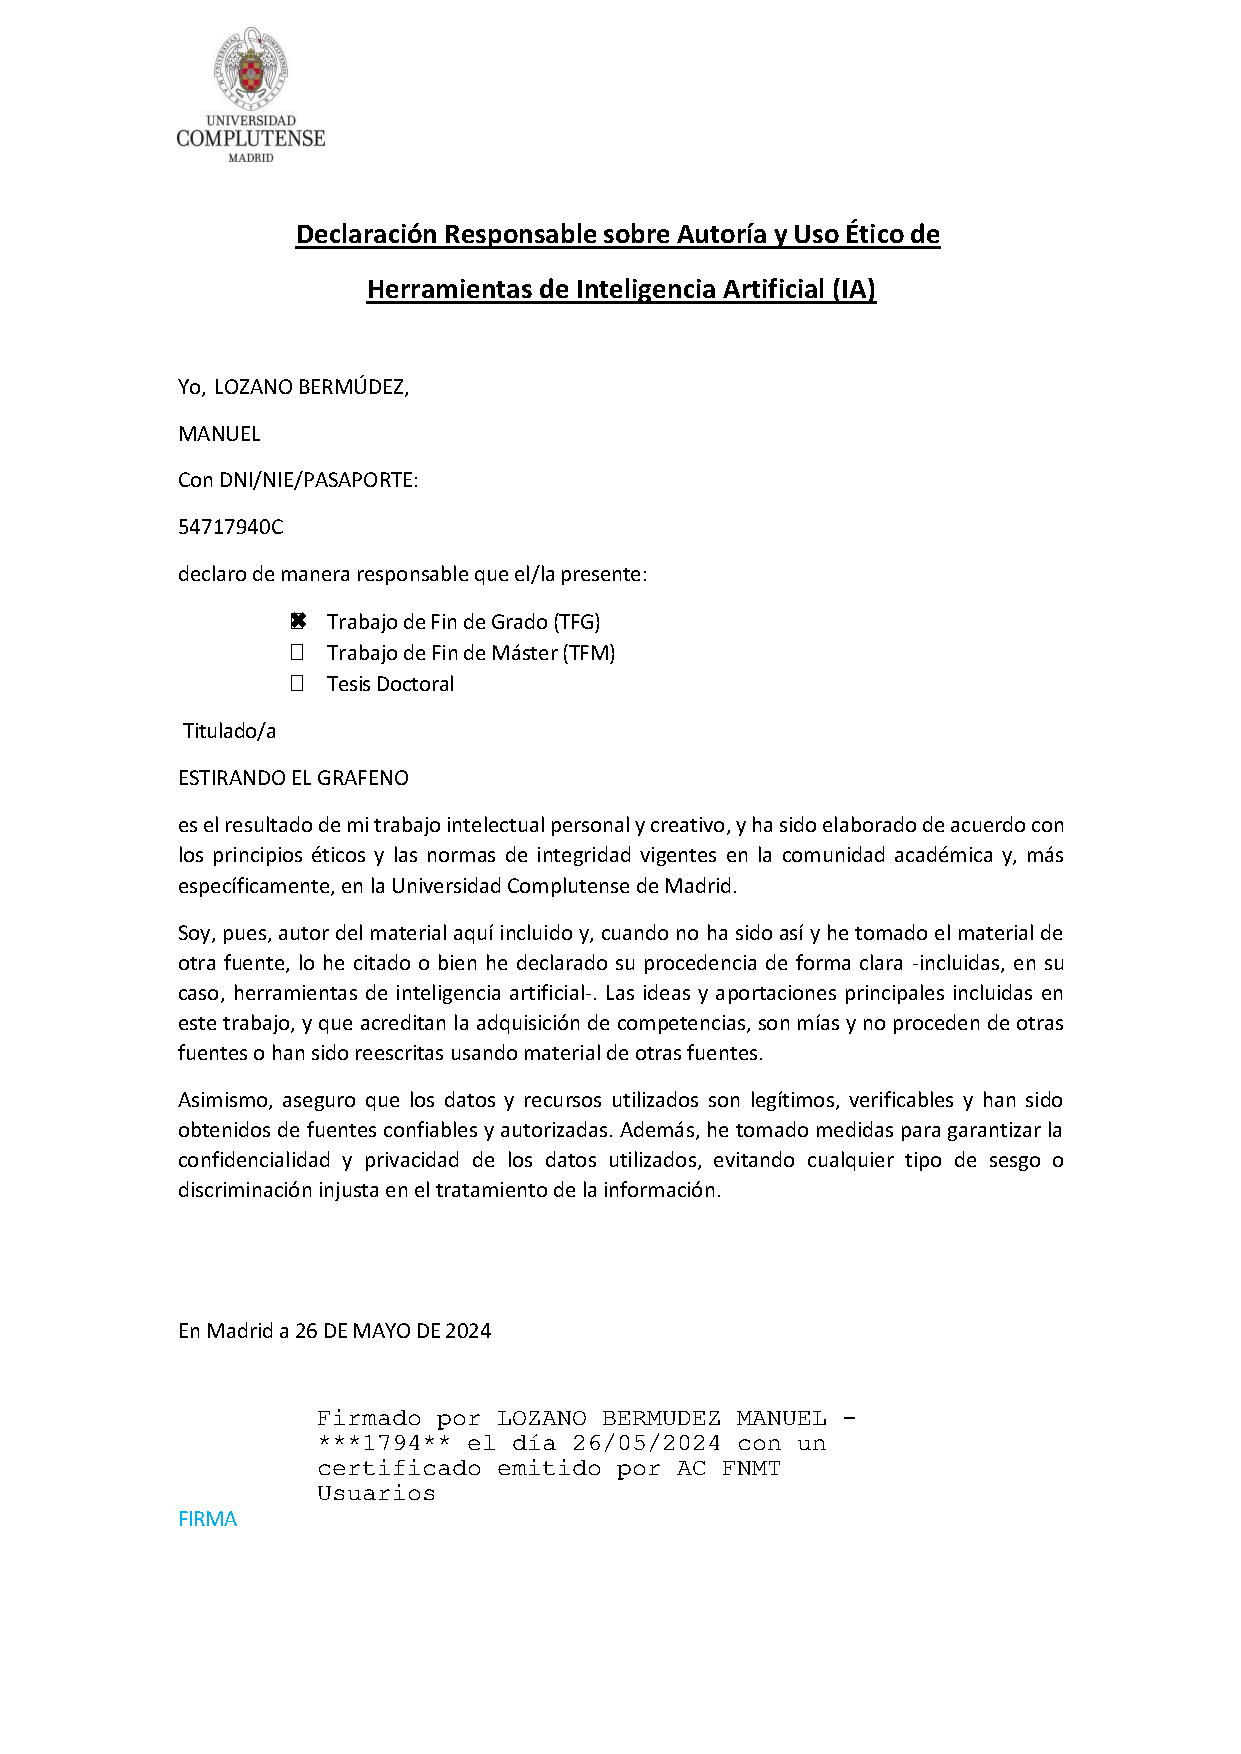
\includepdf{declaracion-responsable-sobre-autoria-y-uso-etico-de-ia_signed.pdf}

% \coffeestainA{0.9}{0.85}{-25}{5cm}{1.3cm}